%!TEX root = ../main.tex
\section{Rime}
\label{sec:design}
% 
\begin{figure}[t]
  \centering
  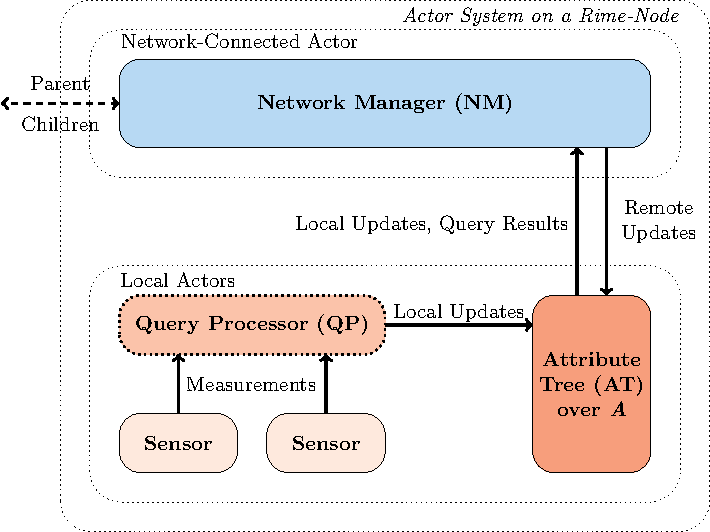
\includegraphics[width=0.48\textwidth]{img/vliot-rime-architecture/vliot-rime-architecture.pdf}
  \caption{Overview of the architecture of Rime and the most important message exchanges between components}
  \label{fig:rime-architecture}
\end{figure}
%
\begin{figure}[t]
  \centering
  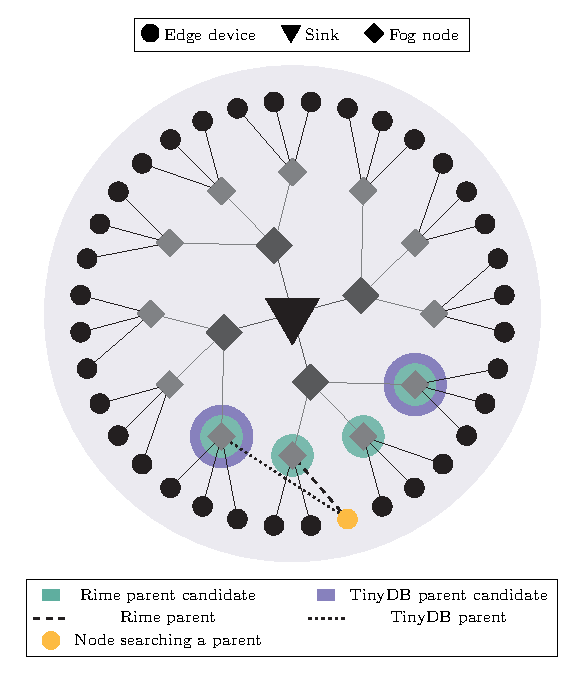
\includegraphics[width=0.48\textwidth]{img/vliot-rime-vs-tinydb/rime-vs-tinydb.pdf}
  \caption{Distance between nodes corresponds to their physical distance. In TinyDB, only nodes in spatial proximity are parent candidates. Rime offers a broader parent pool than TinyDB with its new parent selection.}
  \label{fig:rime-vs-tinydb}
\end{figure}

%
In this section we introduce Rime, a networking component that maintains highly volatile topologies efficiently. Our solution reduces communication costs by exchanging topology information over different gateway nodes and heterogeneous communication schemes.
%\steffen{I think tolerates is not a good term what you mean is can cope with or maintain a highly volatile environment efficiently}
Rime extends the concept of SRTs by introducing an improved parent selection algorithm and a new node tracking policy. At the same time, Rime allows the exchange of topology metadata over different physical areas.
% \steffen{please don't use since so often as it is usually used for time}
%\steffen{is this all? please better sell here and list at least 2 things}
% 
The advantages of Rime are three-fold.
First, by introducing a more efficient parent selection process that reduces the communication and integration overhead, Rime integrates new nodes faster into query processing.
%
Second, to further reduce the amount of exchanged messages, Rime employs a novel tracking policy between nodes. The main goal of the tracking policy is to allow nodes to build an index from their ``known'' nodes. This information is the basis for building and maintaining the extended SRT locally. 
%
Finally, Rime propagates local topology updates within the network, e.g., in the case of node movement. Thus, nodes exchange topology updates with other nodes but do not broadcast them, which reduces the number of messages sent for operations like relocations.
%\steffen{Is this true, so do you actually send less messages? Please make it more explicit what you improve} 
% 
% \steffen{here is a confusion, it sounds like rime is the actor but this part here has to be straighten and more on point}
% 
%
We will present the overall architecture of Rime in Section~\ref{subsec:architecture}, our parent selection algorithm and its details in Section~\ref{subsec:parent-selection}, and the tracking policy in Section~\ref{subsec:tracking-policy}.
% \steffen{again this sounds like rime is the parent selection algorithm}
%

\subsection{Architecture}
\label{subsec:architecture}
Figure~\ref{fig:rime-architecture} outlines the architecture of Rime.
The main goal of Rime is to keep up with a volatile topology and to minimize communication overhead.
% \steffen{maybe one general sentence of what you want to achieve here and what kind of system Rime is}
%Figure~\ref{fig:rime-architecture}
%\steffen{black on green is hard to read + make the fonts larger} shows an overview of Rime and its components over a single node.
Our implementation utilizes the C++ Actor Framework (CAF)~\cite{charousset_native_2013}. 
Rime encapsulates state, e.g., location updates, as part of the actor and models updates as actor messages.
Each Rime node within the network is a distinct actor system, which consists of several local actors and a network-connected actor for communication.
% \steffen{please for all this, refer to parts in the figure where the reader can see this}
Each node contains a \textit{Query Processor (QP)}, multiple sensors, and an \textit{Attribute Tree (AT)}.
% 
A QP is responsible for gathering readings from sensors, perform processing on the readings, and finally update its local AT.
%
The AT holds necessary state, i.e., the current and backup parent, handles to all its children, the local attribute value, and the range of values from the children. In sum, the AT is a superset to the SRT that holds more than just an attribute range. This is to keep the actor implementation simple and spawn as little actors as possible. 
% \johannes{Actually, we spawn an actor for each tree.}
% \steffen{equivalent or the same? please say how it differs by at least one property}
%
The \textit{Network Manager (NM)} serves as the networking gateway that listens for updates and propagates them to other nodes.
During runtime, each AT propagates local updates through the NM to other ATs in other nodes. 
The NM is a stateful actor that is responsible for remote communication and maintaining a key-value store of attributes and handles to the AT.
% 
Furthermore, the NM can react to failures by  monitoring its children and parents. 

% \steffen{so in general you propose a new parent selection algo so you have to constantly point out that this is the most important algorithm for ... such that we really need this, the story here breaks at sever ends, I am unclear why you choose this one}

% The original implementation of TinyDB~\cite{madden2005tinydb} is written as an application on top of TinyOS~\footnote{http://www.tinyos.net/}. 
% TinyOS does not include TinyDB anymore and its API has changed substantially. 
% Since our work is open-source, we provide a framework to the data management community where other researchers can replicate and extend experiments of the same nature~\footnote{repository available as soon as possible}.

\subsection{Parent Selection in Rime}
\label{subsec:parent-selection}
% 
Parent selection is a crucial step in SRTs as it impacts the 
attribute clustering in a specific sub-tree~\cite{madden2005tinydb}.
% 
By clustering, we refer to the value range variance of the attributes stored in an AT.
An AT helps pinpoint nodes
%\steffen{unclear what it means and overall optimal is hard to use here, optimal means you have a min function and want to get the min value, the rest here is too fuzzy} 
that are relevant for a query and avoid unnecessary communication with nodes that do not contain relevant values. 
% \steffen{much too fuzzy, what is unnecessary, when does this happen, etc}
Thus, a small value range in an AT is the main goal when choosing a parent, as it reduces the amount of children when reporting \textit{which} children are relevant to a query.
% \steffen{unclear and hard to follow from the above}

% The two main factors that impact the parent selection process are\steffen{so one is a property or a cost and the other a restriction somehow it is hard to put them on the same level}
% \textit{i)} the quality of candidate parents and \textit{ii)} the selection policy.
Rime uses an \textit{enhanced closest-parent selection policy}, where the best parent candidate 
has the closest attribute value, e.g. location, to the requesting node. This is an extension to
the \textit{closest-parent selection policy} of TinyDB, where updates do not propagate between nodes. 
Essentially Rime exploits the fast network backhaul between gateways to share SRT updates between nodes. 
TinyDB does not offer this possibility due to the cost of constant broadcast communications,
which decreases the life cycle of a battery-powered sensor node.
% \steffen{is this your contribution the policy here or was it there?}
Figure~\ref{fig:rime-vs-tinydb} shows the effects of the different parent selection schemes
between Rime and the original SRT.
%\steffen{ok so is the above yours or the one of tiny db I am confused}. 
The golden node is searching
for a new parent as it just enters the network. Rime provides
a larger pool of parents (green) compared to TinyDB (light blue) as it does not rely only on
nodes that are in physical proximity.
Rime suggests two more potential parents due to the 
exchange of routing information
between nodes that are not in physical proximity. This allows nodes to
continuously update their SRTs without having to perform costly multi-hop broadcast transmissions
to all neighboring nodes.
% \steffen{say explicitly why it is better -- this is still valid why is it better say it explicitly}
%
% \steffen{again be more precise what do you want to reduce, what are the phases, when is it reduced and when not?}
% \steffen{so you introduce 3 concepts above, the candidate parents, the selection policy and the tracking policly but only two of them are explained below}

\textbf{Candidate Parents}
An \textit{ideal} parent candidate has a narrow range of tree-attribute values and is closer to the 
sink than its children. For example, in Figure~\ref{fig:basic-srt}, node \textit{$N_{3}$} reports temperature value around \textit{$(48)$} degrees. There are two candidate parents \textit{$N_{1}$} with value range \textit{$(45, 48)$} and \textit{$N_{2}$} with \textit{$(68, 71)$}. In this case, \textit{$N_{1}$} is a better candidate as it has a narrower value range and its values are closer to \textit{$N_{3}$}.
%
Rime utilizes the parent selection algorithm in Algorithm~\ref{alg:parent-selection} to determine the best parent.
%\steffen{I am confused why explain the same thing again but just differently? I would omit the first one or just merge it}
Algorithm~\ref{alg:parent-selection} starts on a per-request basis from new nodes. The input data are: the distance to an existing parent and the \textit{tree attribute} (\textit{att}) of the new node.
In Lines \texttt{2-8}, the existing node checks all its children and calculates the \textit{euclidean} distance between the tree attributes of the new node and the current child. To this end, we assign the child with the smallest distance as a starting point.
Then, in Line \texttt{9}, the existing
%\steffen{I would always call it new or existing node}
node requests a \textit{random} sibling from its own parent.
The random sibling reply in Line \texttt{10} contains the best candidate child and its distance from the new node to the original random sibling of the existing node. The existing node returns the best child, after comparing its own best child and the best child from the sibling node, in Lines \texttt{11-14}.
This way, Rime returns a larger and better pool of parent candidates for the new node.
% \steffen{I am not sure if I can follow the last sentence-- still true}

% A node initializes the parent selection process based on events, such as a change of its own attribute range or the tree-attribute of its parent.
% % 
% To this end, a node first sends a message to its current parent that contains tree-attribute distance of the node to the current parent.\steffen{I would rather write with first, second, third}
% In Rime, we use \textit{euclidean distance} for all values.
% Afterwards, the parent forwards the message to its own parent, i.e., the \textit{grandparent} of the requesting node. 
% The grandparent tracks all its immediate descendants and computes the distance of each child 
% from the requesting grandchild.
% The grandparent additionally forwards the \textit{parent-selection-request} to a random sibling of its own, if it exists. 
% %
% This forwarding is done to enlarge and broaden the pool of potential parents for the requesting nodes.
% % 
% After the grandparent has received the closest parent from the random sibling, it selects the closest parent out of all candidates. 
% The pool now includes all the children as well as the candidate from the random sibling. 
% Finally, the grandparent forwards the new parent immediately to the grandchild, which subsequently accepts it as its new parent. \steffen{maybe have a figure and explain it with pointers to the figure}
% % 

% We outline our algorithm in Algorithm~\ref{alg:parent-selection}.\steffen{I am confused why explain the same thing again but just differently? I would omit the first one or just merge it}
% The algorithm starts on a per-request basis from new nodes. The input data are: the distance to an existing parent, the \textit{latitude} (\textit{lat}) and \textit{longitude} (\textit{lon}) of the new node, and the \textit{lat,lon} position of the current node.
% In Lines \texttt{3-9}, the node checks all its children, calculates the \textit{euclidean} distance of the new node to the current child. To this end, it will assign the child with the smallest distance as a starting point.
% Then, in Line \texttt{10}, the node requests a \textit{random} sibling from its own parent.
% The random sibling reply, in Line \texttt{11}, contains the best candidate child and its distance from the new node, from the original random sibling of the current node. The node returns the best child, after the comparison
% between its own best child and the best child from the node's sibling, in Lines \texttt{12-15}.
% This way, Rime returns better candidates from the new node, even if these candidates are not included in the local set of children.\steffen{I am not sure if I can follow the last sentence}

\begin{algorithm}[t]
  \SetAlgoLined
  %\SetKwInOut{Input}{Input}
  %\SetKwInOut{Output}{Output}
  \SetKw{Request}{request}
  \SetKw{From}{from}
  \SetKw{Receive}{receive}

  \KwIn{find-better-parent request}
  \KwData{curr\_dist = distance to current parent \\ 
  \hspace{2.7em}att = requesting node tree attribute}
  \KwOut{new parent for requester}
  % \BlankLine    
  \Begin{
      best\_dist = INTEGER\_MAX\;
      best\_idx = -1\;
      % \tcp{find best parent locally}
      \For{child : self.allChildrenNodes}{
          dist = calcEuclideanDist(self.att, child.att)\;
          \If{dist $<$ best\_dist}{
              best\_dist = dist\;
              best\_idx = children.current\_idx\;
          }
      }
      \BlankLine
      \Request random\_sibling \From self.parent\;
      \Receive best\_rand, best\_rand\_dist\;
      % \tcp{best child from random sibling and requesting node's distance to best child}
      \BlankLine
      \uIf{best\_rand\_dist $<$ best\_dist}{
          \Return{best\_rand, best\_rand\_dist}\;
      }
      \Else{
          \Return{children[best\_idx], best\_dist}\;
      }
  }
  \caption{Parent selection at the grandparent of the requesting node}
  \label{alg:parent-selection}
\end{algorithm}

\subsection{Tracking Policy}
\label{subsec:tracking-policy}
Because nodes keep track of several other nodes, the question of 
\textit{which} remote nodes to track arises. Tracking all nodes in the network is infeasible due to scalability reasons, e.g., high message overhead. The main goal of the tracking policy is to decrease the maintenance overhead of ATs by 
reducing the number of tracked nodes.
In order to build an AT within Rime, a node tracks the following:
% steffen{can it even be optimal if it does not track everything?}
First, all nodes require information about their children, i.e., subtree-ranges, and thus track all children. 
Second, a node must know the tree-attribute range of a parent in order to determine how similar it is to its own.
Third, there must be at least one backup node that is required in case of a parent failure. Rime picks the second best parent candidate from the selection process as a backup parent.
% \steffen{say for what}
With the above information, a node is able to perform routing on its own,
%\steffen{what can he decide? be explicit}
without the immediate need to share knowledge to/from others.

Even though Rime allows for routing decisions using local information, it also enables specific nodes to gain knowledge about other nodes in two ways. First, a child 
that selects a new parent sends additional data to the parent, e.g., its IP-address, port, and information about its sensors.
The new parent node tracks the child node by adding its information into its own state.
Second, specific nodes exchange information about other nodes within the network. Exchange only involves specific children, parents, and backup parents and does not work in a broadcast fashion.
%\steffen{I think you said above that you don't do this} 
Nodes maintain local state and data about several other nodes as they are 
able to share it with others on request.
% \steffen{So the main point that will determine if a reviewer will accept or reject your paper is if he sees enough difference between the original SRT in TinyDB and your so please whenever possible point the difference out explicitly}
%\dimi{state here that exchange is only for children nodes, parents, and backup parents}\steffen{again this is contrary to what you said above}
%
This is possible due to the actor-based message exchange of Rime through heterogeneous networks.
% \steffen{I think above you are only talking about networks and not IoT so I would stick to it} 
Given that gateways and intermediate nodes are able to immediately communicate, they do not need to broadcast information to everyone.
%\steffen{I don't get this}
This is in contrast to TinyDB, where nodes broadcast all messages and only 
nodes within antenna range can receive messages. TinyDB is designed for antenna transmissions,
where messages always assume a multi-hop scheme and it is not certain if they will
reach their target. This design decision makes sense for a WSN but is not
enough for a system that is expected to run on top of volatile, heterogeneous networks.
Many core operations in TinyDB, e.g.: message stealing over antennas, are not
feasible in different network configurations. This makes the benefits of the original
broadcast-only system unclear in a modern IoT deployment.
%\steffen{maybe mean receive}
% \steffen{now the 1M dollar question, would we be able use tinydb also with regular network and not antennas and if not why is it still wore than your approach -- still true}

Rime extends the principles behind SRTs in order to remove the
inherent limitations that come with broadcast transmissions.
To this end, nodes in Rime are able to gain topology information to help them to 
form a better AT and reduce the number of exchanged messages.
At the same time, the parent selection and the tracking policy 
reduce communication while propagating updates of the
topology to other locations. These locations are not reachable
using only antenna transmission, contrary to the original SRT design.
The design of Rime is made from the ground-up to exploit
the communication capabilities of IoT infrastructure and bridge the gap between WSNs and the cloud.

% The topology information
% % \steffen{which one?} 
% can originate even from locations where
% it is not possible to communicate using a broadcast scheme.
% %\steffen{???}. 
% Rime moves the concept of SRTs forward and helps simplify
% data management in the IoT by extending knowledge gained from
% WSNs.\steffen{so now you are getting very unstructured and repetitive please check the par again}
